\chapter{Тестирование}

\section{Цели тестирования}

Тестирование в данной работе имеет две цели:

\begin{itemize}

    \item проверка работоспособности процесса после миграции
    \item падение производительности процесса после миграции

\end{itemize}

По причинам описанным в разделе~\ref{syscalls}, использовать \textit{libc} в тестовом приложении нельзя, поэтому тестирование работоспособности процесса после переноса проверяется на небольшом подмножестве системных вызовов (описанных в разделе~\ref{syscalls}).

Падение производительности измеряется по следующим пунктам:

\begin{itemize}
    \item доступ к памяти
    \item арифметические операции
    \item IO
\end{itemize}

Так как не реализована миграция состояния математического сопроцессора, мультимедия и поточного расширений процессора, то падение производительности на арифметических операциях будет будет включать только операции с целыми числами.

\section{Результаты тестирования}\label{results}

\begin{figure}[h]
\center{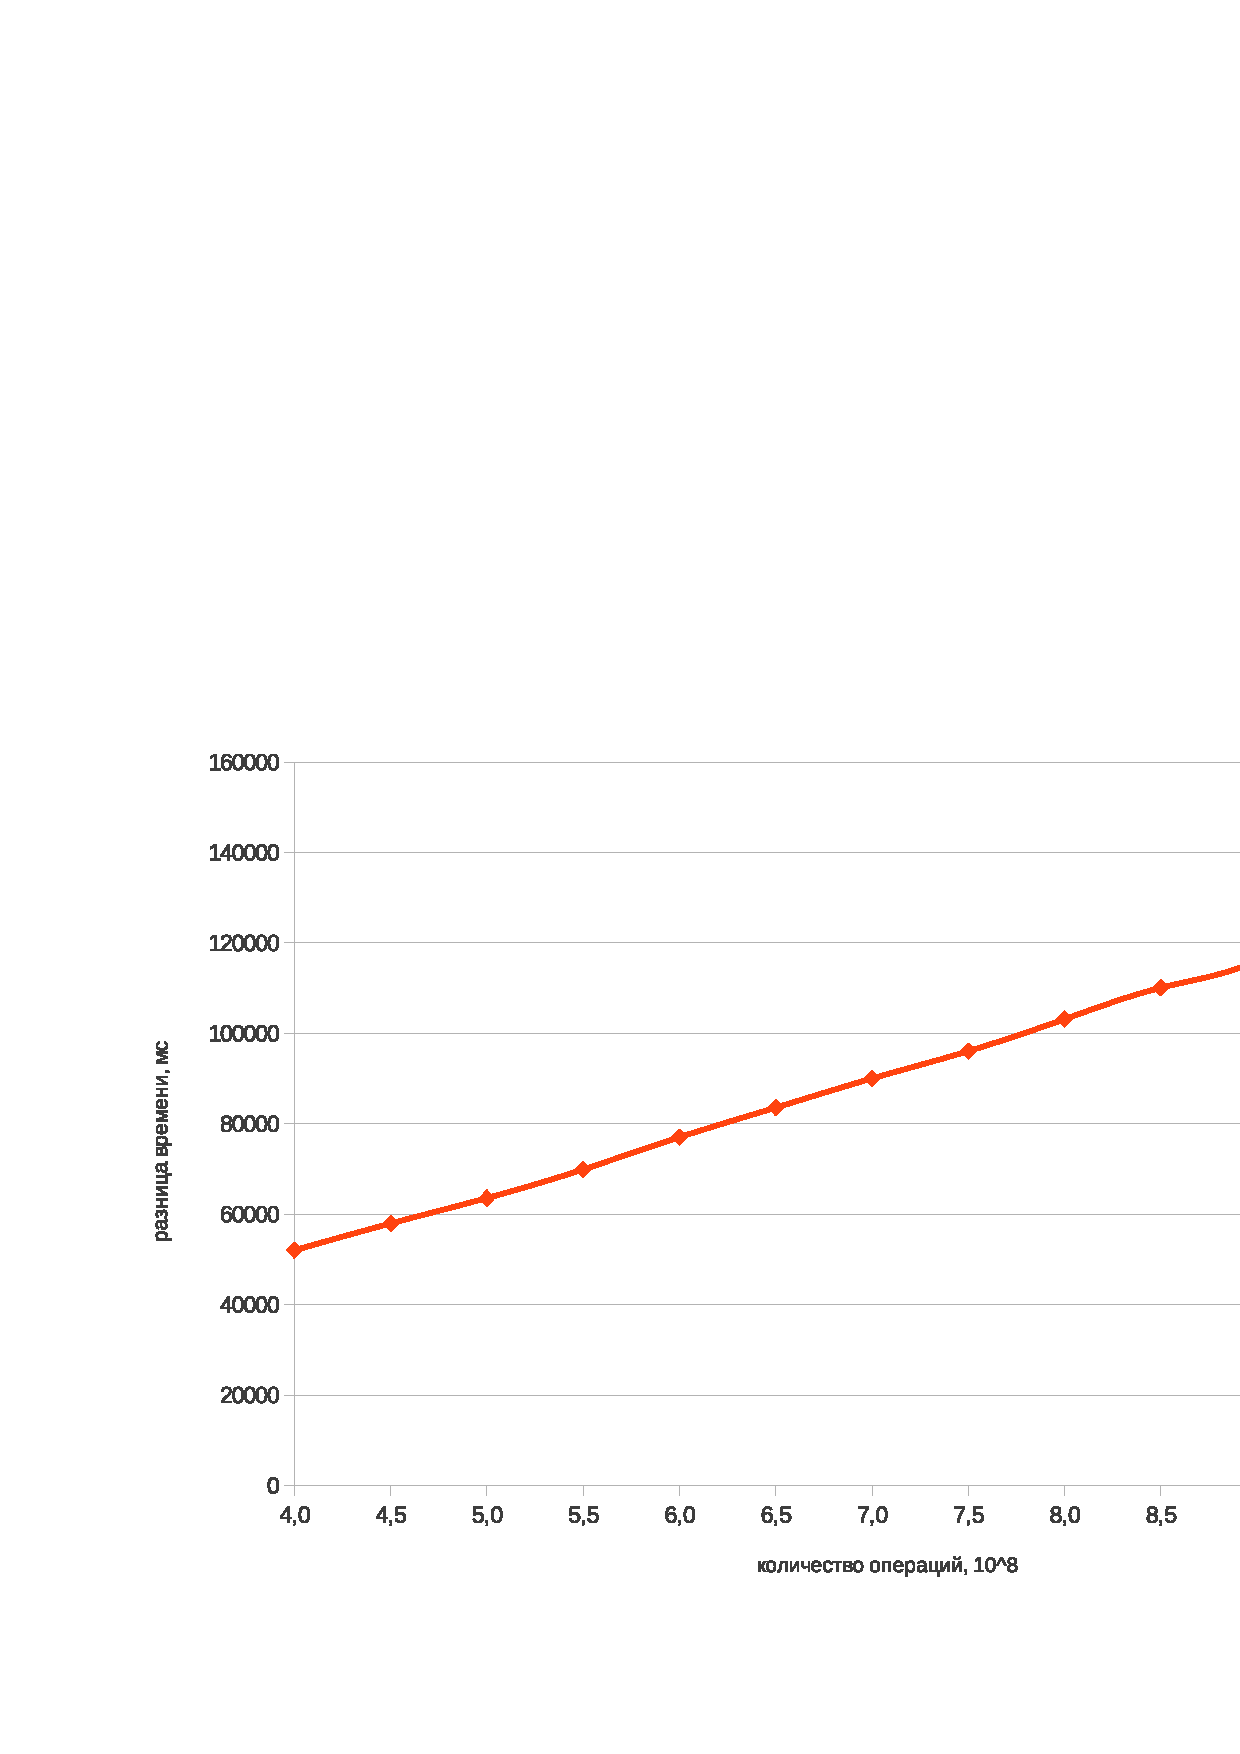
\includegraphics[width=0.8\linewidth]{perf_div}}
\caption{Абсолютные потери производительности на арифметических операциях}
\label{pic:performance_div}
\end{figure}

\begin{figure}[h]
\center{\includegraphics[width=0.8\linewidth]{perf_mem}}
\caption{Абсолютные потери производительности при доступе к памяти}
\label{pic:performance_mem}
\end{figure}

\begin{figure}[h]
\center{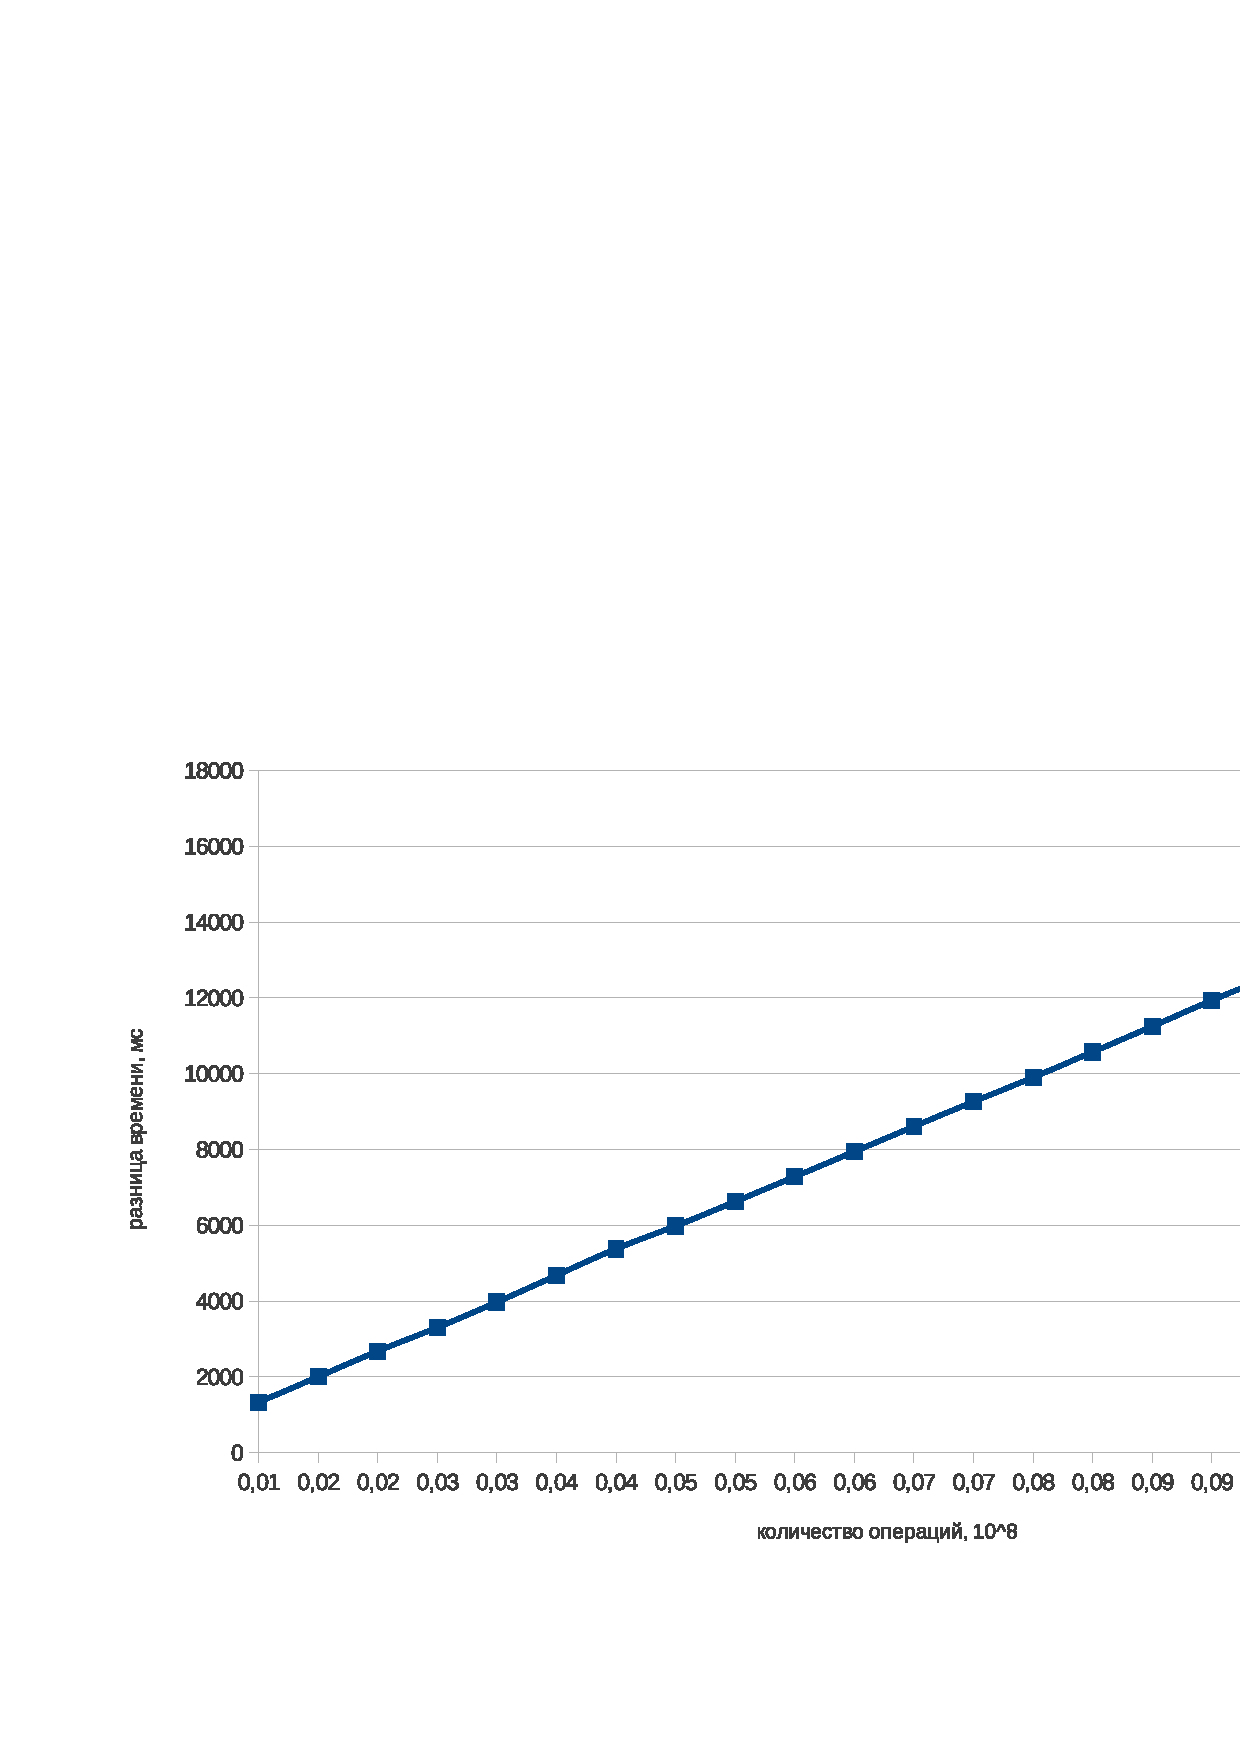
\includegraphics[width=0.8\linewidth]{perf_io}}
\caption{Абсолютные потери производительности при операциях ввода/вывода}
\label{pic:performance_io}
\end{figure}

\begin{table}[h]
\caption{Удельные потери времени на различных операциях}
\label{tbl:preformance_k}
\begin{center}
    \begin{tabular}{|l|c|}
        \hline
        \textbf{Вид операций} & \textbf{Коэффициент, ${mcs}/{ops}$} \\
        \hline
        Доступ к памяти: & 0,009 \\
        Арифметика:      & 0,129 \\ 
        IO:              & 1,269 \\
        \hline
    \end{tabular}
\end{center}
\end{table}

На рис.~\ref{pic:performance_div}, рис.~\ref{pic:performance_mem} и рис.~\ref{pic:performance_io} показаны графики зависимости абсолютных потерь времени от количества операций, на всех графиках прослеживается линейный рост, коэффициенты роста сведены в таблицу~\ref{tbl:preformance_k}
